\documentclass{transcrypto}
\usepackage[utf8]{inputenc}
\usepackage{amsmath}
\usepackage{graphics}

\title{Term Paper by  Team\_Alpha \\ Prince Cipher}
\author{Abinash Acharya (11840050) \\ Thummala Milind Kesar (11841160) \\  Pothukuchi Siddhartha (11840800)}
\institute{Indian Institute of Technology Bhilai , \email{abinasha@iitbhilai.ac.in} \and Indian Institute of Technology Bhilai,\email{thummalam@iitbhilai.ac.in} \and Indian Institute of Technology Bhilai, \email{pothukuchis@iitbhilai.ac.in}}
\begin{document}
\maketitle
\keywords{PRINCE \and Involution \and $\alpha$-reflection \and Integral \and Differential \and S-box \and DDT} 

\begin{abstract}
In this paper, We have described the motivation behind the Prince Cipher and its implementation has been described in detail. Later on, we have discussed some of the practical and theoretical attacks which have been implemented on the cipher. 


\end{abstract}

\section{Introduction}
In recent years, light weight cryptography has drawn a lot of attention. Most of the light weight cryptographic algorithms have been optimized with respect to chip area but such a metric is more specific to application. This particular optimization method is certainly valid in cases where there are tight power and cost constraints (such as passive RFID). But there are many applications require optimization in a different area, for instance instant authentication applications require low-latency encryption and instant response time.Software implementations of virtually all strong ciphers take hundreds or thousands of clock cycles,
making them ill suited for low-latency cryptography. Stream ciphers implemented in hardware are also not a suitable choice for this task because the high number of clock cycles for the initialization phase makes them not suitable for this task. Hence this leaves block ciphers as the remaining option. The low latency implementation becomes difficult because of the iterative nature of block ciphers such as AES. For instance a round based implementation of AES-128 with 10 rounds takes 10 clock cycles to compute the ciphertext. Hence a loop unrolled implementation can be used to compute the ciphertext in a single clock cycle but this comes at a cost of a very long critical path reducing response time and reduced clock frequency. Both are undesirable and there is requirements for new designs for low-latency. This is the motivation behind Prince Cipher.\\
\textbf{The Contributions of Prince Cipher are as follows:}It is optimized with respect to the following features if implemented in hardware:\\
\begin{itemize}
    \item A ciphertext is computed within a single clock cycle, i.e., the cipher does instantaneous encryption.
\item If implemented in modern chip technology, low delays resulting in moderately
high clock rates can be achieved.
\item The hardware costs are moderate (i.e., considerably lower than fully unrolled
versions of AES or PRESENT).
\item Encryption and decryption should both be possible with low costs and overhead.
\end{itemize}
PRINCE compares very favorable to existing ciphers. For the
equal time constraints and technologies, PRINCE uses 6-7 times less area than PRESENT-80 and 14-15 times less area than AES-128. In addition to this,
Prince's design uses about 4-5 times less area than other ciphers.
\section{Cipher Description}
Prince is a 64-bit block cipher with 128-bit key. Instead of treating the cipher as matrix in AES, in Prince the data is treated as a 1D array. The 128-bit key expanded to 196-bit by the following simple method:\\
\begin{center}
    $(k_0||k_1) = (k_0||k'_0||k_1) := (k_0||k_0>>>1) \oplus (k_0>>63||k_1)$
\end{center}
Prince uses FX construction.$k_0$ and $k_1$ are used as whitening keys whereas $k_1$ is the 64-bit key for a 12-round block cipher referred to as PRINCE$_{CORE}$\\
\begin{center}
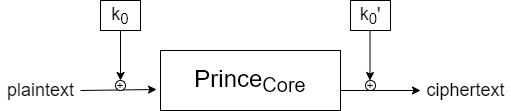
\includegraphics[scale=0.5]{Cipher.jpg} \\ \\
\end{center}
\textbf{PRINCE$_{CORE}$}: The encryption of PRINCE$_{CORE}$ is depicted below.\\
\begin{center}
    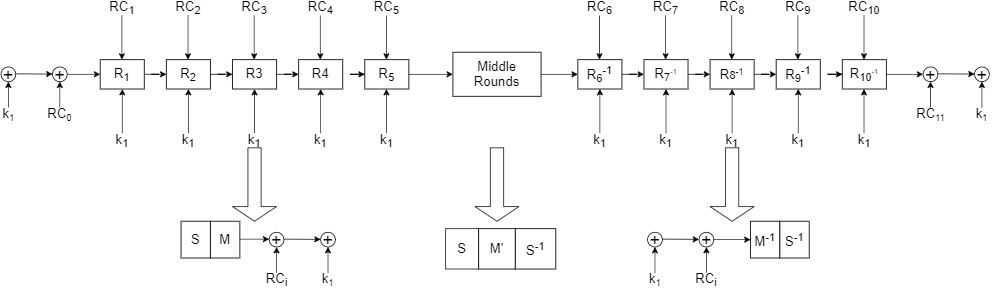
\includegraphics[scale=0.5]{Prince-12-Round.JPG}
\end{center}\\
Each round of PRINCE$_{CORE}$ consists of key addition, an SBOX layer, linear layer and the addition of a round constant.\\
\noindent
\textbf{k$_i$ add:}Each round uses key addition which is simple xor with 64-bit subkey.\\

\noindent
\textbf{S-Layer:}The cipher uses 4-bit Sbox given as follows:\\ \\
\begin{center}
    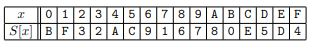
\includegraphics[]{S-box.JPG} \\ \\
\end{center}

\noindent
\textbf{The Matrices M/$M'$ layer:}This layer provides diffusion and is multiplication of the state with a 64x64 matrix.\\

\noindent
\textbf{RC$_i$ add:}In this, a 64-bit round constant is xored with the state.\\


\begin{center}
    \begin{tabular}{|c||c|}
         \hline
         $RC_0$ & 0000000000000000 \\
         \hline
         $RC_1$ & 13198a2e03707344 \\
         \hline
         $RC_2$ & a4093822299f31d0 \\
         \hline
         $RC_3$ & 082efa98ec4e6c89 \\
         \hline
         $RC_4$ & 452821e638d01377 \\
         \hline
         $RC_5$ & be5466cf34e90c6c \\
         \hline
         $RC_6$ & 7ef84f78fd955cb1 \\
         \hline
         $RC_7$ & 85840851f1ac43aa \\
         \hline
         $RC_8$ & c882d32f25323c54 \\
         \hline
         $RC_9$ & 64a51195e0e3610d \\
         \hline
         $RC_10$ &  d3b5a399ca0c2399 \\
         \hline
         $RC_11$ & c0ac29b7c97c50dd \\
         \hline
        \end{tabular}
\end{center}
More details of the various components are in the implementation section.\\

\section{Implementation:}\\
\subsection{Choosing the Sbox:}\\
This layer eliminates any linearity so that the cipher cannot be expressed as a system of any number of linear equations. The cost of the sbox (area and critical path) is a substantial part of the overall cost and hence it is important to choose an Sbox that reduces cost. However to ensure security, the choice of sbox should ensure the following criteria:
\begin{itemize}
    \item Maximal probability of a differential = 1/4
\item There are 15 differentials with probability 1/4.
\item Maximal absolute bias of a linear approximation = 1/4.
\item There are 30 linear approximations with absolute bias 1/4.
\item Each of the 15 non-zero component functions has algebraic degree 3.
\end{itemize}
There are 8 sboxes fulfilling this criteria and the discussion summarizes to choosing an sbox from the 8 possible choices.\\
\subsection{$\alpha$ Reflection Property:}
An interesting aspect of the Prince Cipher is it's symmetric nature. The Round Constants are such that for $0\leq i \leq 11$, RC$_i$ $\oplus$ RC$_{11-i}$ = constant. This is the constant $\alpha$ which in our case takes the value c0ac29b7c97c50dd. RC$_0$ is 0 and RC$_1$,..RC$_5$ are derived from the fractional part of $\pi$.\\
From this property and because $M'$ is an involution,one can deduce that inverse of PRINCE$_{CORE}$ parametrized with k is equivalent to PRINCE$_{CORE}$ parametrized with k$\oplus\alpha$. This property of PRINCE$_{CORE}$ is called $\alpha$ reflection property. Hence for a key $(k_0||k'_0||k_1)$,
\begin{center}
    $D_{(k_0||k'_0||k_1)}(.)=E_{(k'_0||k_0||k_1\oplus\alpha)}(.)$
\end{center}
Hence for decryption one has to do a cheap change and then use the exact same circuit as that for encryption.
\subsection{Key Expansion:}
 In PRINCE, the 128-bit key ($k_{0}||k_{1}$) is expanded to get a 192 bit key ($k_{0}||k'_{0}||k_{1}$) by using:
\begin{align*}
    (k_{0}||k_{1}) \xrightarrow{}(k_{0}||P(k_{0})||k_{1})
\end{align*}
This expansion is based on the FX construction and it is done to prevent attacks which can be done by partially guessing the key $k_1$(since this key is used in all 12 rounds of the cipher).
 Hence it would be preferred that each pair of subkeys among $k_{1}$ and the quantities ($k_{0} \oplus k_{1} $) and ($k^{'}_{0} \oplus k_{1}$) takes all the $2^{128}$ possible values when ($k_{0}||k_{1}$) belongs to the whole set of 128-bit words so that we don't restrict the value of the expanded key . Alternatively,it can be said that  the set of all triples ($k_{0}||P(k_{0})||k_{1}$) should correspond to an MDS code of length 3 and size $2^{128}$ over $F^{64}_{2}$. In other words  both $x\xrightarrow{} P(x)$ and $x \xrightarrow{} x \oplus P(x)$ should be permutations of $F^{64}_{2}$.
\\
Thus, a hardware-favaourable choice for P such that both$ P$ and $P \oplus Id$ are permutations is
\begin{align*}
    P(x) = (x \gg 1) \oplus (x \gg 63) ,
\end{align*}
$P(x_{63}, . . . , x_{0}) = (x_{0}, x_{63}, . . . , x_{2}, x_{1} \oplus x_{63})$. Then, it can be easily verified that $P(x) = 0$ (resp. $P(x) = x$) has a unique solution.
\subsection{The Linear Layer:}\\
The Linear Layer consists of 2 segments/operations - one is the Shift Rows and the other is the M' layer. Both of them are used in continuation of each other. But, in the middle rounds, the M'-layer is used separately. Due to this, to preserve the symmetry of the cipher, M'-layer must be an involution. On the other hand, the M-layer doesn't need to be an involution since it is present in the forward rounds and the backwards rounds in the exact opposite order so as to reverse the effect while decryption. \\ Furthermore, we have to achieve diffusion and that's why shift rows has been used along with the M'-layer in the forward and backward rounds. \\
The Shift Rows operation behaves similar to that of AES shift rows and it shuffles the nibbles in the following manner : \\
\begin{table}[!ht]
\begin{tabular}{|l|l|l|l|l|l|l|l|l|l|l|l|l|l|l|l|}
\hline
0 & 1 & 2  & 3  & 4 & 5 & 6  & 7 & 8 & 9  & 10 & 11 & 12 & 13 & 14 & 15 \\ \hline
0 & 5 & 10 & 15 & 4 & 9 & 14 & 3 & 8 & 13 & 2  & 7  & 12 & 1  & 6  & 11 \\ \hline
\end{tabular}
\end{table} \\
In order to minimize the cost of the implementation, the matrix used in the M'-layer should have as few number of ones as possible to facilitate easier and quicker computation.\\ However, at the same time, there must be at least 16 active S-boxes in 4 successive rounds for the sake of security and diffusion. Hence, to strike a balance, the number of ones per row and per column has been kept as 3 and the following 4 x 4 matrices can be used as frameworks for the larger 64 x 64 matrix M'. \\ \\
$M_{0}=$
\begin{bmatrix} 
0 & 0 & 0 & 0\\
0 & 1 & 0 & 0\\
0 & 0 & 1 & 0\\
0 & 0 & 0 & 1\\
\end{bmatrix}
\quad
$M_{1}=$
\begin{bmatrix} 
1 & 0 & 0 & 0\\
0 & 0 & 0 & 0\\
0 & 0 & 1 & 0\\
0 & 0 & 0 & 1\\
\end{bmatrix}
\quad
$M_{2}=$
\begin{bmatrix} 
1 & 0 & 0 & 0\\
0 & 1 & 0 & 0\\
0 & 0 & 0 & 0\\
0 & 0 & 0 & 1\\
\end{bmatrix}
\quad
$M_{3}=$
\begin{bmatrix} 
1 & 0 & 0 & 0\\
0 & 1 & 0 & 0\\
0 & 0 & 1 & 0\\
0 & 0 & 0 & 0\\
\end{bmatrix}
\\
Now, we construct two 16 x 16 matrices $\Vec{M^{(0)}}$ and $\Vec{M^{(1)}}$ where each row and column is a chosen permutation of the 4 matrices listed above ($M_{0},M_{1},M_{2},M_{3}.$) in such a manner that the 16 x 16 matrices which we obtain are involutions which implies they are inverses of themselves. \\ \\
$\Vec{M^{(0)}}=$
$\begin{bmatrix} 
M_{0} & M_{1} & M_{2} & M_{3}\\
M_{1} & M_{2} & M_{3} & M_{0}\\
M_{2} & M_{3} & M_{0} & M_{1}\\
M_{3} & M_{0} & M_{1} & M_{2}\\
\end{bmatrix}$
\quad
$\Vec{M^{(1)}}=$
$\begin{bmatrix} 
M_{1} & M_{2} & M_{3} & M_{0}\\
M_{2} & M_{3} & M_{0} & M_{1}\\
M_{3} & M_{0} & M_{1} & M_{2}\\
M_{0} & M_{1} & M_{2} & M_{3}\\
\end{bmatrix}$
\\ \\
We use the 16 x 16 matrices that have been derived above along the diagonal  of the 64 x 64 matrix i.e. our M'-layer \\ All other values will be kept as zero.  \\ \\
 $\begin{pmatrix} 
    M_0 & 0 & 0 & 0\\
    0 & M_1 & 0 & 0\\
    0 & 0 & M_1 & 0\\
    0 & 0 & 0 & M_0\\
\end{pmatrix}$
\\ \\
Due to this construction, the matrix M' is an involution having a total of $2^{32}$ fixed points. Fixed points refer to those states which remain unchanged even after the M'-layer operates on them. \\ 
We will use this fact later when we study the differential attack. \\
\section{Practical Attacks}
\subsection{Integral Attacks}
\subsubsection{4-Round Attack}
Here, we attack the round-reduced version of PRINCE. For even-rounds, we have added same number of rounds before and after the middle rounds while for odd-rounds, we have added one additional round at the beginning. \\
In this Attack, we begin with 1 active nibble (out of 16) in the plaintext and guess the key through partial decryption making use of the fact that all nibbles are balanced after 3.5 rounds. 
Therefore, We begin with 1 Nibble having the ALL property and rest having the Constant Property and end up with all Balanced nibbles at the end of 3.5 rounds. Below is a representation of the property : \\ \\

\begin{tabular}{|c|c|c|c|}
    \hline
    A & C & C & C \\
    \hline 
    C & C & C & C \\
     \hline
    C & C & C & C \\
    \hline
    C & C & C & C \\
    \hline
\end{tabular}
$\xrightarrow{S,M}$
\begin{tabular}{|c|c|c|c|}
    \hline
     $A^8$ & C & C & C \\
    \hline 
    C & C & C &  $A^8$ \\
     \hline
    C & C &  $A^8$ & C \\
    \hline
    C &  $A^8$ & C & C \\
    \hline
\end{tabular}
$\xrightarrow{S,M'}$
\begin{tabular}{|c|c|c|c|}
    \hline
    $A^8$ &  $A^4$ &  $A^4$ &  $A^8$\\
    \hline 
    $A^4$ &  $A^4$ &  $A^4$ &  $A^4$  \\
     \hline
    $A^4$ &  $A^4$ &  $A^4$ &  $A^4$ \\
    \hline
    $A^4$ &  $A^8$ &  $A^8$ &  $A^4$\\
    \hline
\end{tabular}
$\xrightarrow{S^{-1},M^{-1}}$ \\ \\ \\ \\ 
\begin{tabular}{|c|c|c|c|}
    \hline
    B &  B &  B &  B\\
    \hline 
    B &  B &  B &  B  \\
     \hline
    B &  B &  B &  B \\
    \hline
   B &  B &  B &  B\\
    \hline
\end{tabular} \\ \\

Note :- (1) $A^8$ - Nibble taking 8 distinct values 
       (2) $A^4$ - Nibble taking 4 distinct values \\ \\
As you can see above, every nibble becomes balanced after 3.5 rounds.
But this balanced property may get destroyed after the 4th round S-box transforms it. So, in order to recover the key, we guess (k0' $\oplus$ k1) (since these are the final key additions) and partially decrypt the ciphertext through the last S-box and check whether all the nibbles are balanced. \\
For the purpose of accuracy(to decrease the effect of wrong key guesses), we take 5 sets of $2^4$ plaintexts each and identify that value of (k0' $\oplus$ k1) which exists in correct key guesses for all  the sets. \\
After recovering (k0' $\oplus$ k1), the next part of the attack is to recover k1.\\
Now, we take 5 sets of $2^4$ plaintexts starting with 4 active nibbles as it has been shown in the 2nd diagram. \\
We remove the 4th round by doing Xoring the ciphertext with the recovered (k0' $\oplus$ k1). Then, we invert the linear layer and for all possible key guesses of nibbles in k1, we partially decrypt further through 1 S-box. \\
A correct nibble key guess is one which gives a balanced nibble. \\
Next, we identify a value of k1 which exists among the correct key guesses in all the 5 sets of plaintexts taken. \\
Next, we xor the recovered (k0' $\oplus$ k1) and k1 to obtain k0'.\\
From k0',we can easily obtain k0 by doing a set of linear operations. \\  \\
\underline{Data and Time Complexity} \\ \\
We choose 5 sets of $2^4$ plaintexts twice, once for the recovery of k0' $\oplus$ k1 and again for the recovery of k1. \\
So, Total Data complexity = $2\times5\times2^4 \approx 2^7$ \\
Each S-box transformation is a single operation. \\
For each plaintext, S-box is called 16 times (once for each nibble).\\ 
We have in total $2\times5\times2^4$ plaintexts. \\
Therefore, time complexity of this attack = $16\times2\times5\times2^4 \approx 2^{11}$
\subsubsection{5-Round Attack}
This attack is  an extension of the 4-Round Attack. \\ 
In this Attack, we begin with 1 active nibble (out of 16) in the plaintext and guess the key through partial decryption of 1.5 rounds making use of the fact that all nibbles are balanced after 3.5 rounds. 
Therefore, We begin with 1 Nibble having the ALL property and rest having the Constant Property and end up with all Balanced nibbles at the end of 3.5 rounds.  \\
But this balanced property may get destroyed after the 4th round and 5th round S-box transform it. So, in order to recover the key, we guess a complete column of (k0' $\oplus$ k1) (since these are the final key additions) and partially decrypt the ciphertext through the last S-box and M-layer and again guess a nibble of k1 , decrypt it through 1 more S-box and check whether all the nibbles are balanced. \\
For the purpose of accuracy(to decrease the effect of wrong key guesses), we take 6 sets of $2^4$ plaintexts each and identify that value of (k0' $\oplus$ k1) which exists in correct key guesses for all  the sets. \\
After recovering (k0' $\oplus$ k1), the next part of the attack is to recover k1.\\
Now, we use the same 6 sets and remove the  5th round completely by using the guessed value of k0' $\oplus$ k1 and guess each nibble of k1 to partially decrypt the 4th round state through 1 S-box.    \\
A correct nibble key guess is one which gives a balanced nibble. \\
Next, we identify a value of k1 which exists among the correct key guesses in all the 6 sets of plaintexts taken. \\
Next, we xor the recovered (k0' $\oplus$ k1) and k1 to obtain k0'.\\
From k0',we can easily obtain k0 by doing a set of linear operations. \\ 
\section{Differential Attacks}
\subsection{Some Important Points to Keep in Mind}
The difference is studied between the trail from middle to plaintext and trail from middle to ciphertext. Round reduced version for this analysis has a construction n-x-n where the details are as follows: \\ \\
(1) Pre-whitening with $k_1$ and $RC_0$ \\
(2) n forward rounds \\
(3) the middle part ($S, M', S^{-1}$) \\
(4) n backward rounds \\
(5) post whitening with $k_1$ and $RC_{11}$ \\ \\
There are $2^8$ columns (4 nibbles) each which pass through $M^(0)$ and $M^(1)$ respectively without any change.
So, there are $(2^8)^4$ states (64-bit values) which can go through the M' layer without any effect. \\ 
Therefore, these $2^{32}$ states which can go through the middle round unchanged. (since M' layer won't affect the state and S and $S^{-1}$ will cancel out each other's effect.) \\ \\
\underline{S-box Analysis} \\  \\ 
The Difference Distribution Table for the S-box of PRINCE is as follows : \\ \\
\begin{tabular}{|c|c|c|c|c|c|c|c|c|c|c|c|c|c|c|c|c|c|}
\hline
in/out & 0 & 1 & 2 & 3 & 4 & 5 & 6 & 7 & 8 & 9 & a & b & c & d & e & f & No. of solutions \\
\hline
0 & 16 & 0 & 0 & 0 & 0 & 0 & 0 & 0 & 0 & 0 & 0 & 0 & 0 & 0 & 0 & 0 & 1 \\
\hline
1 & 0 & 4 & 0 & 0 & 2 & 0 & 2 & 0 & 4 & 2 & 0 & 2 & 0 & 0 & 0 & 0 & 6\\
\hline
2 & 0 & 2 & 0 & 4 & 0 & 0 & 0 & 2 & 2 & 0 & 0 & 0 & 0 & 4 & 2 & 0 & 6 \\
\hline
3 & 0 & 0 & 0 & 0 & 0 & 2 & 2 & 0 & 2 & 2 & 2 & 2 & 2 & 0 & 0 & 2 & 8\\
\hline
4 & 0 & 2 & 2 & 4 & 2 & 2 & 0 & 0 & 2 & 0 & 2 & 0 & 0 & 0 & 0 & 0 & 7 \\
\hline
5 & 0 & 0 & 2 & 2 & 0 & 2 & 0 & 2 & 0 & 2 & 0 & 2 & 2 & 2 & 0 & 0 & 8 \\
\hline
6 & 0 & 0 & 2 & 2 & 0 & 2 & 2 & 0 & 0 & 2 & 0 & 2 & 0 & 0 & 4 & 0 & 7 \\
\hline
7 & 0 & 0 & 2 & 0 & 0 & 0 & 2 & 0 & 2 & 0 & 4 & 0 & 0 & 2 & 2 & 2 & 7 \\
\hline
8 & 0 & 0 & 2 & 0 & 4 & 2 & 0 & 0 & 2 & 2 & 0 & 2 & 0 & 2 & 0 & 0 & 7 \\
\hline
9 & 0 & 0 & 2 & 2 & 0 & 0 & 0 & 0 & 0 & 2 & 2 & 0 & 4 & 2 & 0 & 2 & 7 \\
\hline
a & 0 & 0 & 0 & 2 & 2 & 4 & 0 & 4 & 2 & 0 & 0 & 0 & 0 & 0 & 0 & 2 & 6\\
\hline
b & 0 & 2 & 0 & 0 & 4 & 0 & 0 & 2 & 0 & 0 & 0 & 2 & 2 & 0 & 2 & 2 & 7\\
\hline
c & 0 & 4 & 0 & 0 & 0 & 2 & 2 & 0 & 0 & 0 & 2 & 2 & 2 & 0 & 2 & 0 & 7 \\
\hline
d & 0 & 2 & 0 & 0 & 0 & 0 & 0 & 2 & 0 & 4 & 2 & 0 & 0 & 2 & 2 & 2 & 7 \\
\hline
e & 0 & 0 & 2 & 0 & 0 & 0 & 4 & 2 & 0 & 0 & 0 & 2 & 2 & 2 & 0 & 2 & 7 \\
\hline
f & 0 & 0 & 2 & 0 & 2 & 0 & 2 & 2 & 0 & 0 & 2 & 0 & 2 & 0 & 2 & 2 & 8 \\
\hline
\end{tabular} \\ \\ \\
The last column shows the number of possible output differences for each of the input differences. 
\\ 
The Difference Distribution Table for the inverse S-box of PRINCE is as follows : \\ \\
\begin{tabular}{|c|c|c|c|c|c|c|c|c|c|c|c|c|c|c|c|c|c|}
\hline
in/out & 0 & 1 & 2 & 3 & 4 & 5 & 6 & 7 & 8 & 9 & a & b & c & d & e & f & No. of solutions \\
\hline
0 & 16 & 0 & 0 & 0 & 0 & 0 & 0 & 0 & 0 & 0 & 0 & 0 & 0 & 0 & 0 & 0 & 1 \\
\hline
1 & 0 & 4 & 2 & 0 & 2 & 0 & 0 & 0 & 0 & 0 & 0 & 2 & 4 & 2 & 0 & 0 & 6 \\
\hline
2 & 0 & 0 & 0 & 0 & 2 & 2 & 2 & 2 & 2 & 2 & 0 & 0 & 0 & 0 & 2 & 2 & 8 \\
\hline
3 & 0 & 0 & 4 & 0 & 4 & 2 & 2 & 0 & 0 & 2 & 2 & 0 & 0 & 0 & 0 & 0 & 6 \\
\hline
4 & 0 & 2 & 0 & 0 & 2 & 0 & 0 & 0 & 4 & 0 & 2 & 4 & 0 & 0 & 0 & 2 & 6 \\
\hline
5 & 0 & 0 & 0 & 2 & 2 & 2 & 2 & 0 & 2 & 0 & 4 & 0 & 2 & 0 & 0 & 0 & 7 \\
\hline
6 & 0 & 2 & 0 & 2 & 0 & 0 & 2 & 2 & 0 & 0 & 0 & 0 & 2 & 0 & 4 & 2 & 7 \\
\hline
7 & 0 & 0 & 2 & 0 & 0 & 2 & 0 & 0 & 0 & 0 & 4 & 2 & 0 & 2 & 2 & 2 & 7 \\
\hline
8 & 0 & 4 & 2 & 2 & 2 & 0 & 0 & 2 & 2 & 0 & 2 & 0 & 0 & 0 & 0 & 0 & 7 \\
\hline
9 & 0 & 2 & 0 & 2 & 0 & 2 & 2 & 0 & 2 & 2 & 0 & 0 & 0 & 4 & 0 & 0 & 7 \\
\hline
a & 0 & 0 & 0 & 2 & 2 & 0 & 0 & 4 & 0 & 2 & 0 & 0 & 2 & 2 & 0 & 2 & 7 \\
\hline
b & 0 & 2 & 0 & 2 & 0 & 2 & 2 & 0 & 2 & 0 & 0 & 2 & 2 & 0 & 2 & 0 & 8 \\
\hline
c & 0 & 0 & 0 & 2 & 0 & 2 & 0 & 0 & 0 & 4 & 0 & 2 & 2 & 0 & 2 & 2 & 7 \\
\hline
d & 0 & 0 & 4 & 0 & 0 & 2 & 0 & 2 & 2 & 2 & 0 & 0 & 0 & 2 & 2 & 0 & 7  \\
\hline
e & 0 & 0 & 2 & 0 & 0 & 0 & 4 & 2 & 0 & 0 & 0 & 2 & 2 & 2 & 0 & 2 & 7   \\
\hline
f & 0 & 0 & 0 & 2 & 0 & 0 & 0 & 2 & 0 & 2 & 2 & 2 & 0 & 2 & 2 & 2 & 8  \\
\hline
\end{tabular} \\ \\ \\ \\ 
\underline{Note} \\
If we sum up the numbers in the solutions column for each of the tables, the result is 106. So,  256 pairs of input and outputs correspond to 106 possible output differences. \\ 
Average non-zero value in the DDT (for both S\_box and S\_inv) = 256/106 = 2.415 (We will use this in the attacks) \\  
\subsection{2 Round Inside-Out Attack}
% Here, we study the differential trail from the middle rounds and observe how the difference changes in corresponding positions between the  forward  and backward rounds. \\
% \underline{Observation} \\
% There are $2^8$ columns (4 nibbles) each which pass through $M^(0)$ and $M^(1)$ respectively without any change.
% So, there are $(2^8)^4$ states (64-bit values) which can go through the M' layer without any effect. \\ 
% Therefore, these $2^{32}$ states which can go through the middle round unchanged. (since M' layer won't affect the state and S and $S^{-1}$ will cancel out each other's effect.) \\
We will use these states as the initial difference starting from the middle rounds. \\
Below is a representation of the trail : \\ \\
\begin{center}
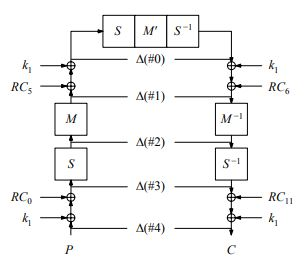
\includegraphics[scale=0.75]{DC.JPG} \\ \\
\end{center}

The differential trail is as follows: \\ \\
$\xrightarrow[p=2^{-32}]{S^{-1},M',S}  0 \xrightarrow[p=1]{\oplus k1 \oplus RC_5/RC_6} \alpha \xrightarrow[p=1]{M^{-1}} \beta \xrightarrow[p=1]{S^{-1}} \gamma \xrightarrow[p=1]{\oplus k1 \oplus RC_{11}/RC_0} \gamma \oplus \alpha $ \\ \\
\textbf{How the Difference propagates:}\\
We see that the difference here is not between two plaintexts rather it is between intermediate stages which are symmetrical about $SM'S^{-1}$ and finally between the plaintext and ciphertext. It is denoted at different stages by $\triangle(\#0),\triangle(\#0),...$. The propagation through various components is as follows.
\begin{itemize}
    \item \textbf{Key and Round Constant Addition} :- We already know that addition of key on both sides will not affect the difference as key is same. However the round constants differ by $\alpha$ and hence we observe $\triangle(\#0)=\alpha\oplus\triangle(\#1)$
    \item \textbf{M or $M^{-1}$} :- This applies diffusion and hence difference changes as both sides are diffused differently, however we can obtain with probability 1 the value of resulting difference.
    \item \textbf{Sbox} :- This is the non linear component and hence we can only be certain with a probability of how the difference will propagate based on DDT.
\end{itemize}
The attack is as follows : \\ \\
\begin{enumerate}
    \item We choose $2^{32}$ plaintexts and query their corresponding ciphertexts from the oracle. From the Observation, we made there will be at least one plaintext-ciphertext pair for which $\Delta(\#0)$=0. ($\Delta(\#0)$ is the difference between the states before the middle rounds and after the middle rounds. This is the starting point of our differential trail) 
    \item We know that : \\
    $\gamma_i \oplus \alpha =  P_i \oplus C_i$  \\
    So, we calculate $\gamma_i$ for all the ($P_i,C_i$) pairs. \\
    \item $\alpha$ gets transformed into $\beta$ through the $M'^{-1}$ layer. By applying the $M'^{-1}$ layer to $\alpha$=(c0ac || 29b7 || c97c || 50dd), we get $\beta$= (42a3 || 356a || 5d3a || 0fe3) with probability 1. \\
    Again, for $\beta$, we can derive the number of output differences possible by multiplying the number of solutions derived (for each hexadecimal character in $\beta$) in the table above for the inverse S-box. This value comes out to be $6 \times 8 \times ... \times 6 \approx 2^{41.38}$.
    All these  possible output differences are potential values of $\gamma_i$. We filter out all the ($P_i,C_i$) pairs for which $\gamma$ doesn't belong to the above potential values.
    Expected number of pairs remaining after filtration = $2^{32} \times 2^{-64} \times 2^{41.38} = 2^{9.38}$  
    \item We find 4 hexadecimal characters a,b,c,d for each nibble of $P_i$ such that $a \oplus b = \gamma \xrightarrow{S} \beta= c \oplus d$  holds. For each of the 106 output differences, there are 256 values possible. Average number of solutions for the above equation (for each nibble) = $\frac{256}{106}$ = 2.415 \\ \\
    For all 16 nibbles, total number of solutions possible = $(2.415)^{16} \approx 2^{20.35}$ \\ 
    So, for each plaintext $P_i$, we have these many solutions denoted by $(\#3)_i$ (These are the solutions for $\gamma_i$). We refer to each of these solutions by  $(\#3)^j_i$. \\
    For each of these solutions, we guess the value of $K_1$ using the relation below : \\
    $(K_1)^j_i = P_i + RC_0 + (\#3)^j_i $ \\
    For 1 plaintext, we have $2^{20.35}$ potential values. So, for $2^{9.38}$ plaintexts remaining after filtration, we have $2^{20.35} \times 2^{9.38} = 2^{29.73}$ possible values.  
    \item For each guessed key $(K_1)^j_i$, we encrypt any plaintext other than $P_i$ and check if the calculated ciphertext (using guessed key) matches with that given by the oracle. If they are equal, our key guess is correct.
\end{enumerate}
Here, the Data and memory complexity are  $2^{32}$ (since we are querying and storing these many (P,C) pairs). \\
Time Complexity = $2^{32} + 2^{29.73} \approx 2^{32}$
\subsection{4 Round Inside-Out Attack}
For the 4 Round Inside-Out Attack we make a construction very similar to the 2-round Inside-Out Attack as follows:\\
\begin{center}
    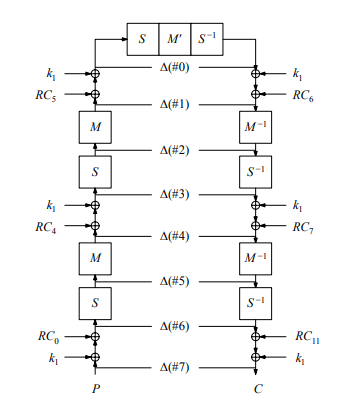
\includegraphics[scale=0.5]{image.png}
\end{center}
We can see that it is a 2-x-2 construction. Now the differential trail is as follows:\\
\begin{center}
    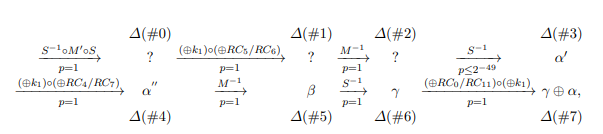
\includegraphics[scale=0.6]{pic.png}
\end{center}
Here \\
\begin{align*}
    \alpha ' = (c0a\cdot|| 29\cdot7 || c\cdot7c||\cdot0dd)\\
    \alpha '' = (000\cdot ||00\cdot0||0\cdot00||\cdot000)\\
    \beta=(000\cdot ||000\cdot||000\cdot||000\cdot)\\
    \gamma=(000\cdot||000\cdot||000\cdot||000\cdot)
\end{align*}
The attack is as follows:\\
\begin{itemize}
    \item We take $2^{48}$ pairs of plaintexts, ciphertexts denoted by ($P_i,C_i$) and for each pair we compute $\gamma_i$. By observing the trail we can notice that \begin{equation*}
        \gamma_i \oplus \alpha = P_i \oplus C_i
    \end{equation*}. This is because they are seperated only by key addition and $RC_0,RC_1$ which differ by $\alpha$. Since 16 bits in $\alpha '$ are not specifies, we expect to have 1 pair of plaintext, ciphertext such that $\triangle(\#3)=\alpha '$
    \item Now we match 48 bits to be 0 and since such a high number of bits is matched we expect only few plaintexts and ciphertexts to remain.\\
    \item Now to go from $\triangle \#6$ to $\triangle \#5$ we need to derive from the remaining plaintexts the solutions a,b,c,d $\in \{0,1\}^4$ such that $a\oplus b =\gamma \xrightarrow{S} c \oplus d = \beta$. We need to consider all 16 possible values per nibble for each of the 12 nibbles in the leftmost column of the state $(\#6)_i^j$. For the remaining 4 nibbles there are $(2^{1.27})^4$ which $2^{5.08}$ solution per pair. Hence we need to get $2^32^{48}2^{5.08}\approx 2^{56.08}$ potential values for $(\#6)_i^j$
    \item The candidate key is computed as $(K_1)_i^j=P_i\oplus RC_0\oplus(\#6)_i^j$ for each possible potential value of the state $(\#6)_i^j$.
    \item Encypt $P_j$ using key guess and verify if it is the same as $C_j$ obtained by querying the oracle such that i$\neq$ j. Hence this will eliminate the false positives.
\end{itemize}
Hence the complexity of the attack is $2^{56.08}$, the memory complexity is $2^{48}$ for storing the plaintext, ciphertexts and the data complexity is $2^{48}$ for choosing the plain texts.
\section{$\alpha$-Reflection Attack}
As mentioned earlier, one explicit feature of PRINCE is the $\alpha$-reflection property of $PRINCE_{core}$. But, not amazingly, the development we tend to used for getting this feature additionally has structural properties, as well as an involutional middle spherical, and care needs to be taken once planning a cipher with such a structure. In this section, we tend to analyze the influence of this construction on the protection of the cipher. particularly, we tend to have an interest within the questionable profile of the core cipher, i.e., in the sequence of the lengths of all cycles within the decomposition of $PRINCE_{core}$.
\\ The first strategy for exploiting some data on the profile of the core cipher is the following. If the decomposition of the core cipher is independent of the key, then then this decomposition can be used as a distinguishing property for recovering some information on the whitening keys. The only illustration of this sort of attack is once the core cipher is an involution, i.e. $\alpha$ = zero Indeed, the attack bestowed by Dunkelmanet permits to recover the total of the 2 whitening keys$(k_{0} \oplus k_{2})$in the FX construction once F is AN involution. This attack uses the actual fact that for 2 plaintext-ciphertext pairs$(m, c)$ and $(m_{0},c_{0})$ connected by $m_{0}=E^{-1}_{k_{0},k_{1},k_{2}}(m \oplus k_{0} \oplus k_{2})$it holds that $m \oplus c=m^{′} \oplus c^{′}$.Indeed
\begin{align*}
    m^{'}\oplus c^{'} = E^{−1}_{k_{0},k_{1},k_{2}}(m \oplus k_{0}\oplus k_{2}) \oplus m \oplus k_{0} \oplus k_{2}
    \\
    =k_{0} \oplus F^{-1}_{k_{1}}(m \oplus k_{0}) \oplus m \oplus k_{0} \oplus k_{2}
    \\
    =F_{k_{1}}(m \oplus k_{0}) \oplus m \oplus k_{2}
    \\
    = m \oplus c
\end{align*}
here the last-but-one equality uses that $F_{k_{1}}$ is an involution. Thus, plaintext-
ciphertext pairs (m, c) and ($m^{'} , c^{'}$ ) such that $c^{'} = m \oplus k_{0} \oplus k_{2}$ can be easily 
detected. Such a collision can be found if the attacker has access to $2^{\frac{n+1}{2}}$  known
plaintext-ciphertext pairs, and it provides the value of $(k_{0} \oplus k_{2} )$. Moreover, in
the particular case of PRINCE , $k_{2}$ is related to $k_{0}$ by $k_{2}$ = $P (k_{0} )$ where $x \xrightarrow[]{} x \oplus P (x)$ is a permutation (see Section 3.3). Therefore, the whitening key $k_{0}$ can be deduced from $(k_{0} \oplus k_{2} )$ in this case. It follows that, when the core cipher is an involution, the whole key can then be recovered with time complexity $2^{k}$ (corresponding to an exhaustive search for $k_{1}$ ) and data complexity $2^{\frac{n+1}{2}}$ .\\
This type of attack can be generalized to the case where the profile of the core cipher does not rely on $k_{1}$ : since $PRINCE_{core}$ has a reasonable block size, its cycle structure may well be precomputed nd so used as a distinctive property for ($k_{0} \oplus k_{2}$ ). Indeed, the profile of $E_{k_{0} ,k_{1},k_{2}}: m \xrightarrow[]{} k_{2} \oplus F_{k_{1}}(m \oplus k_{0})$
depends on $(k_{0} \oplus k_{2})$ only. It follows that, for each n-bit word $\delta$, we could compute
one or a few cycles of $x \xrightarrow[]{} F_{k_{1}}(x \oplus k_{ 0}  \oplus k_{2} \oplus \delta)$ in a chosen-plaintext scenario where the attacker knows a sequence of plaintext-ciphertext pairs $(m_{i} , c_{i} )$ with $m_{i+1} = c_{i} \oplus \delta$. a sound candidate for $(k_{0} \oplus k_{2} )$ is a value $\delta$ which leads to a cycle having a length that seems within the precomputed profile of $F_{k_{1}}$ . We checked whether the cycle structure of $PRINCE_{core}$ has some peculiarities which do not depend on its key. based on the technique employed by Biryukov for analyzing involutional ciphers, we can observe the profile of the reduced version of $PRINCE_{core}$ with 4 Sbox layers where we keep the symmetry around the middle does not depend on the key.Actually, this reduced version can be written as  
\begin{align*}
G =(R^{−1} o Add_{k_{1} \oplus \alpha})o (S^{-1} o M_{0} o S) o (Add_{k_{1}} o R_{5})
\end{align*}
\\
where R5 corresponds to $\Re5$ without the key addition. Since $(S^{−1} o M_{0} o S)$ is an involution, the cycle structure of $Add_{k_{1} \oplus \alpha} o (S^{-1} o M_{0} o S)$ $Add_{k_{1}}$ depends on $\alpha$ solely and not on $k_{1}$. Its profile then remains unchanged once a right composition with $R_{5}$ and a left composition with its inverse. However, this property doesn't hold any longer once an extra round is enclosed since succeeding key addition $Add_{k_{1} \oplus \alpha} o G o Add_{k_{1}}$ modifies the cycle structure of G in an exceedingly manner that depends on the values G, and not solely on its profile. Therefore, it seems that the antecedently mentioned attack strategy doesn't apply if $PRINCE_{core}$ contains over six Sbox layers. 
\\
In the light of the previous analysis, a additional relevant attack technique consists in using the very fact that the core cipher might have a peculiar cycle decomposition for a few weak keys. as an example, if there exists some weak keys $k_{1}$ for which $PRINCE_{core}$ is an involution, then this class of keys can be detected from the knowledge of $2^{\frac{n+1}{2}}$ pairs of plaintext-ciphertext by counting the number of collisions for $m \oplus c$. And the technique that we've got antecedently described also recovers the whitening key. it's price noticing that this attack applies to DESX and permits to find the employment of the four weak keys of DES that DES is an involution. an identical weakness would seem if,  in $PRINCE_{core}$, we have used two subkeys $k_{1}$ and $k^{'}_{1}$ in turn as round keys. Keeping the remaining structure of $PRINCE_{core}$ results in the following relation
\begin{align*}
    F^{-1}_{k_{1}||k_{1}^{'}}=F_{(k_{1}^{'} \oplus \alpha|| k_{1} \oplus \alpha)}
\end{align*}
However, this has serious – and fascinating – consequences for the protection of the ensuing cipher. For the category of keys such as $k_{0}=k_{1} \oplus \alpha$, it holds that
\begin{align*}
    F^{-1}_{k_{1}||k_{1}^{'}}=F_{k_{1}||k_{1}^{'}}
\end{align*}
 , the core cipher is an involution. This category of weak keys will then be simply detected.It then seems that some specific related-key distinguishers for the core cipher is also exploited for detecting the corresponding category of keys. To be terribly clear, we have a tendency to don't consider related key-attacks here within the classical sense of enlarging the facility of an adversary. But without a careful alternative, the development we used for implementing the -reflection property might end in key-recovery attacks for certain weak-key categories, as presently because the core cipher is vulnerable to related key-attacks
\section{Conclusion}
In this paper, we studied the complete implementation of PRINCE. We have implemented it in python in the file PrinceCipher.py. 
We studied its various components including the S-box and the linear layer. 
We have generated the Difference distribution tables for both the S-box and its inverse in the files DDT\_S\_box.py and DDT\_S\_inv.py 
We have performed some analysis on both the tables and we have showed the same in this paper.\\
We have studied different attacks on PRINCE including the 2-round differential attack, the 4-Round differential attack,etc.
Additionally, we have implemented a practical attack on PRINCE which is a 4-Round Integral Attack in the file 4roundintegral\_2.py 
We nominate this attack performed for Brownie points since we have implemented the complete attack and successfully recovered the key.
Again, we also have studied the 5-Round Integral Attack. 
At the end, we have studied a very popular full fledged attack on the Prince Cipher known as the $\alpha$-reflection attack. 
\section{References}
\begin{itemize}
    \item On the security of the core of PRINCE against biclique and differential cryptanalysis [\href{http://eprint.iacr.org/2012/712}{link}]
    \item Truncated differential cryptanalysis of PRINCE [\href{https://onlinelibrary.wiley.com/doi/full/10.1002/sec.1213}{link}]
    \item PRINCE – A Low-latency Block Cipher for Pervasive Computing Applications [\href{https://eprint.iacr.org/2012/529.pdf}{link}]
    \item Practical Attacks on the Round-reduced PRINCE [\href{https://eprint.iacr.org/2015/245.pdf}{link}]
    \item Reflection Cryptanalysis of PRINCE-like Ciphers  [\href{https://www.iacr.org/archive/fse2013/84240065/84240065.pdf}{link}]
    \item Security Analysis of PRINCE [\href{https://eprint.iacr.org/2015/372.pdf}{link}]
    
    
    
\end{itemize}
\end{document}

